\section{问题二的建模与求解}

\subsection{数据预处理}

与问题一类似地, 对于样本缺失值过多的特征(超过 80\%) 进行剔除, 共剔除了 20 个特征列, 同时对于处理后的数据集中存在缺失值的样本进行剔除共剔除了 547 行。对于余下的样本的92个特征进一步的处理,筛选出更有代表性特征。

\subsubsection{以相关性筛除特征}

对于处理后的生命体征指标,筛选出相关性较大的特征,将它们关联为一种特征能够极大的减少模型中的冗余信息和噪声,删除较大相关性的特征可以帮助提高下面建立模型的泛化能力和解释能力。以相关性来筛除特征,首先需对数据集进行归一化处理,为了避免数值问题,利用min-max标准化方法对数据采用min-max标准化进行处理,定义数据为:$Z=\{{{z}_{1}},{{z}_{2}},\cdots ,{{z}_{n}}\}$,min-max标准化的公式为:

\begin{equation}
    z_{i}^{'}=\frac{{{z}_{i}}-{{z}_{\min }}}{{{z}_{\max }}-{{z}_{\min }}}.
\end{equation}

处理好的数据表示为:${{Z}^{'}}=\{z_{1}^{'},z_{2}^{'},\cdots ,z_{n}^{'}\}$。斯皮尔曼相关系数可以根据以下公式进行计算:

\begin{equation}
    \rho =1-\frac{6\sum\limits_{i=1}^{n}{d_{i}^{2}}}{n({{n}^{2}}-1)}.
\end{equation}
其中$n$为样本容量,$\rho$为相关系数,${{d}_{i}}$为样本的两个变量中对应的数据次序的等级差(等级差指的是将样本按从小到大排序后规定等级,如果数值相同,则将它们所在的位置取算术平均)。计算不同特征之间的相关系数,筛除掉高度相关的特征,以减少数据集中的冗余信息和降低模型过拟合的风险。本文基于Pandas的corr()函数来计算相关系数,并认为相关系数的绝对值大于0.7是高度相关的特征,计算各个特征之间的相关性这里删除相关性大于0.7的特征列(通过相似性处理最终得到49个特征代表整个生命体征,总共删除了43个特征)。

\subsubsection{基于主成分分析法的数据降维}

上面虽然得到49个生命体征,但是对于分析不同药组之间的具体的显著性差异来说,生命体征特征仍然偏多会导致分析难度大,不利于准确的分析出其中的差异性,需要对数据特征进行进一步的降维处理,基于主成分分析法的数据降维是一种常见的数据降维技术,通过将多个相关性高的变量合并成少数几个不相关的变量(即主成分),从而降低数据维度,提高数据处理和分析的效率。

本文采用PCA降维方法,通过线性变换将原始数据映射到新的空间中,从而得到降维后的数据。在这个新的空间中,原始数据中的冗余信息被消除,只保留了最重要的特征。设筛选后的数据构成一个$\overrightarrow{x}={{\left( {{x}_{1}},{{x}_{2}},\cdots ,{{x}_{p}} \right)}^{T}}$为一个$p$维随机变量,并假定二阶矩阵存在,记均值向量为:

\begin{equation}
    \overrightarrow{\mu }=E\left( \overrightarrow{x} \right).
\end{equation}
协方差矩阵为:

\begin{equation}
    \sum =V\left( \overrightarrow{x} \right).
\end{equation}
下式进行线性变换:

\begin{equation}
    \left\{ \begin{matrix}
       {{y}_{1}}={{a}_{11}}{{x}_{1}}+{{a}_{12}}{{x}_{2}}+\cdots +{{a}_{1p}}{{x}_{p}}=\overrightarrow{a}_{1}^{T}\overrightarrow{x}  \\
       {{y}_{2}}={{a}_{21}}{{x}_{1}}+{{a}_{22}}{{x}_{2}}+\cdots +{{a}_{2p}}{{x}_{p}}=\overrightarrow{a}_{2}^{T}\overrightarrow{x}  \\
       \cdots   \\
       {{y}_{p}}={{a}_{p1}}{{x}_{1}}+{{a}_{p2}}{{x}_{2}}+\cdots +{{a}_{pp}}{{x}_{p}}=\overrightarrow{a}_{p}^{T}\overrightarrow{x}  \\
    \end{matrix}\right.
\end{equation}

约束条件有:

\begin{enumerate}
  \item $\overrightarrow{a}_{i}^{T}\overrightarrow{a}=a_{1i}^{2}+a_{2i}^{2}+\cdots +a_{pi}^{2}=1\left( i=1,2,\cdots ,p \right)$
  \item 当时$i>1$,$\operatorname{cov}\left( {{y}_{i}},{{y}_{j}} \right)=0\left( j=1,2,\cdots ,i-1 \right)$,即${{y}_{i}}$与${{y}_{j}}$不相关。;
  \item $\operatorname{var}\left( {{y}_{i}} \right)=\underset{{{\overrightarrow{a}}^{T}}\overrightarrow{a}=1,\operatorname{cov}\left( {{y}_{i}},{{y}_{j}} \right)=0}{\mathop{\max }}\,\operatorname{var}\left( {{\overrightarrow{a}}^{T}}\overrightarrow{x} \right)\left( j=1,2,\cdots ,i-1 \right)$
\end{enumerate}

设${{\lambda }_{1}},{{\lambda }_{2}},\cdots ,{{\lambda }_{p}}\left( {{\lambda }_{1}}\ge {{\lambda }_{2}}\ge \cdots \ge {{\lambda }_{p}}\ge 0 \right)$为$\sum $的特征值,${{\overrightarrow{t}}_{1}},{{\overrightarrow{t}}_{2}},\cdots ,{{\overrightarrow{t}}_{p}}$为相应的一组正交单位特征向量,$\overrightarrow{x}={{\left( {{x}_{1}},{{x}_{2}},\cdots ,{{x}_{p}} \right)}^{T}}$的主成分就是以$\sum $的特征向量为系数的线性组合,它们互不相关,线性组合的方差为$\sum $的特征值。

当${{\overrightarrow{a}}_{1}}={{\overrightarrow{t}}_{1}}$时,$V\left( {{y}_{1}} \right)=\overrightarrow{a}_{1}^{T}\sum {{\overrightarrow{a}}_{1}}={{\lambda }_{1}}$达到最大值,所求的${{y}_{1}}=\overrightarrow{t}_{1}^{T}\overrightarrow{x}$就是第一主成分。如果第一主成分所含的信息不够多,不足以代表原始的$p$个向量,则需要再考虑使用${{y}_{2}}$。为了使${{y}_{2}}$所含的信息与${{y}_{1}}$不重叠,要求$\operatorname{cov}\left( {{y}_{i}},{{y}_{j}} \right)=0$。当${{\overrightarrow{a}}_{2}}={{\overrightarrow{t}}_{2}}$时,$V\left( {{y}_{2}} \right)=\overrightarrow{a}_{2}^{T}\sum {{\overrightarrow{a}}_{2}}={{\lambda }_{2}}$达到最大值,所求的${{y}_{2}}=\overrightarrow{t}_{2}^{T}\overrightarrow{x}$就是第二主成分。与此类似,可以再定义第三主成分,直至第$p$主成分.一般来说,$\overrightarrow{x}$的第$i$主成分是指约束条件下的${{y}_{i}}=\overrightarrow{t}_{i}^{T}\overrightarrow{x}$。

记$\overrightarrow{y}={{\left( {{y}_{1}},{{y}_{2}},\cdots ,{{y}_{p}} \right)}^{T}}$,主成分向量$\overrightarrow{y}$与原始向量$\overrightarrow{x}$的关系为$\overrightarrow{y}={{T}^{T}}\overrightarrow{x}$,其中$\overrightarrow{T}={{\left( {{\overrightarrow{t}}_{1}},{{\overrightarrow{t}}_{2}},\cdots ,{{\overrightarrow{t}}_{p}} \right)}^{T}}$。

第$i$主成分在总方差$\sum\limits_{i=1}^{p}{{{\lambda }_{i}}}$中的比例${{\lambda }_{i}}/\sum\limits_{i=1}^{p}{{{\lambda }_{i}}}$称为主成分的贡献率,第一主成分的贡献率最大,表明它解释原始变量的能力最强,${{y}_{2}}\sim {{y}_{p}}$的解释能力依次减弱.主成分分析的目的在于减少变量的个数,因而一般不会使用所有$p$个主成分,忽略一些带有较小方差的主成分不会给总方差带来太大的影响。

前$m$个主成分的贡献率之和在总方差中的比例$\sum\limits_{i=1}^{m}{{{\lambda }_{i}}}/\sum\limits_{i=1}^{p}{{{\lambda }_{i}}}$称为主成分${{y}_{1}},{{y}_{2}},\cdots ,{{y}_{m}}$的累计贡献率,它表明了${{y}_{1}},{{y}_{2}},\cdots ,{{y}_{m}}$解释原始变量的能力。通常去较小(相对于$p$)的$m$,可使得累计贡献率达到一个较高的百分比,此时${{y}_{1}},{{y}_{2}},\cdots ,{{y}_{m}}$可替代$\sum $,从而达到降维的目的,而信息的损失不多。

PCA通过构建新的主成分来实现降维,本文基于Scikit-Learn库的PCA函数实现主成分分析法。首先初始化pca模型,并通过参数n\_components指定降维后的特征维度,当前特征空间共49个列向量。接着调用fit\_transform方法对原始数据进行降维,并基于matplotlib绘制主成分方差解释比例图:

\begin{figure}[H] % 这个H不要动!
	\centering % 不要动!
	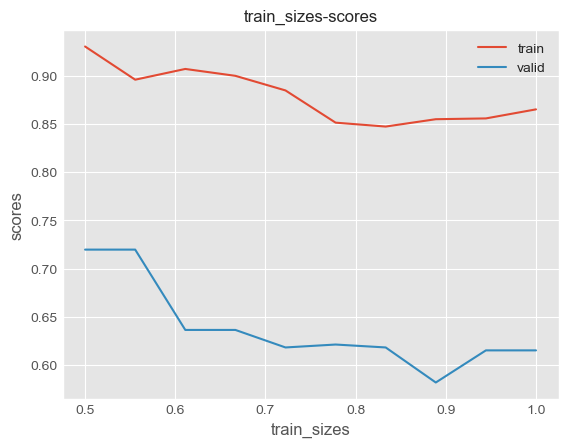
\includegraphics[width=0.95\textwidth]{5.png} 
	\caption{主成分方差解释比例图} 
	\label{Fig.main5} 
\end{figure}

该图显示了每个主成分的方差解释比例。为了使得到的主成分能够较为完整的表示原信息,本文基于图中信息选择将49个特征降维成15个主成分——显然降维为15个主成分时可成分解释比例超过0.8,丢失的信息较少,故使用这15个主成分特征能够较好反映生命指标数据的信息。

由于降维后的数据不再表示原生命体征的意义,其本身不再具有具体的实际意义,却蕴含原生命指标的信息。同时处理得到的主成分不再具有原始数据的列名,因此重新给它们分配了新的列名,将这前15个主成分依次命名$\left\{ 1,2,3,\cdots ,15 \right\}$,同时与镇静药名称、性别、年龄、身高、体重、是否吸烟、是否酗酒、有无PONV、有无晕动史11个特征构成含有新的数据集。这里欲全面科学的探究出不同药组的差异性情况,因此考虑了患者其他的情况,不失一般性。下面利用这15个能够代表原生命体征的主成分直接与不同的药组进行进一步的差异性分析。

\subsection{药组对于生命体征数据的差异性探究}

利用上面15个主成分来研究新药组和原有药物组在生命体征数据方面是否表现出显著差异,本文通过独立样本t检验、Mann-Whitney U检验来研究药组对于生命体征数据的15个主成分是否具有显著性,进而得出结论。

\subsubsection{正态性检验}

欲进行独立样本的假设检验,需先进行正态性检验。依题意,有:

\begin{enumerate}
  \item 原假设${{H}_{0}}$:样本数据服从正态分布;
  \item 备择假设${{H}_{1}}$:样本数据不服从正态分布;
\end{enumerate}

计算了一个统计量:

\begin{equation}
    {{K}^{2}}={{S}^{2}}+{{V}^{2}}.
\end{equation}
其中,$S$是样本偏度,$V$是样本峰度.

对基于主成分分析降维出的15个主成分特征进行正态性检验,基于Scipy库中的normaltest函数进行正态性检验。对这15个主成分进行正态性检验,通过其返回值p值表示数据是否符合正态分布,p小于0.05,则拒绝原假设,认为数据不符合正态分布,只能进行Mann-Whitney U检验;否则接受原假设,认为数据符合正态分布,可以进行独立样本t检验。正态性检验的结果如下表:

\begin{table}[H]
    \centering  
    \caption{正态性检验结果}
    \begin{tabular}{c c c}  
    	\toprule[1.5pt]  
    	正态分布 & 非正态分布 \\  
    	\midrule[1pt]    
    	5、6、7、9、12~~~ & 1、2、3、4、8、10、11、13、14、15 \\ 
    	\toprule[1.5pt]  
    \end{tabular}  
\end{table} 

从上表可以清楚的得到满足正态分布能够进行独立样本检验的主成分为第 5、6、7、9、12 主成分,不满足正态分布进行非参数检验的是第1、2、3、4、8、10、11、13、14、15。

\subsubsection{独立样本的参数、非参数检验}

基于以上正态检验的结果对这15个特征分别进行参数或非参数检验。对第5、6、7、9、12主成分分别进行独立样本T检验,先将标签数据根据是否使用镇静药分为两组,然后对这两组数据进行独立样本t检验。t检验用于判断两组数据之间的均值是否存在显著性差异,独立样本T检验的原理是基于$T$统计量,利用和$t$值和$p$值来判断这两个样本是否显著不同。

\begin{enumerate}
  \item 原假设${{H}_{0}}$:样本数据之间没有显著差异性;
  \item 备择假设${{H}_{1}}$:样本数据之间有显著差异性.
\end{enumerate}
计算公式如下:

\begin{equation}
    t=\frac{{{\overline{x}}_{1}}-{{\overline{x}}_{2}}}{\sqrt{\frac{s_{1}^{2}}{{{n}_{1}}}+\frac{s_{2}^{2}}{{{n}_{2}}}}}.
\end{equation}

\begin{equation}
    p=2\left( 1-{{t}_{{{n}_{1}}+{{n}_{2}}-2}}(|t|) \right).
\end{equation}
其中,${{\overline{x}}_{1}}$和${{\overline{x}}_{2}}$分别表示每个两特征组样本的均值,${{s}_{1}}$和${{s}_{2}}$分别为两组样本的标准差,${{n}_{1}}$和${{n}_{2}}$分别为两组样本的样本量,$t$为检验统计量。${{t}_{{{n}_{1}}+{{n}_{2}}-2}}(|t|)$表示$t$分布的累积分布函数,$|t|$表示$t$值的绝对值。


对第1 、2 、3 、4 、8 、10 、11 、13 、14 、15主成分用Mann-Whitney U进行非参数检验,其原假设为两组独立样本的总体分布相同,备择假设为两组独立样本的总体分布不同。Mann-Whitney U检验的统计量为$U$值,其$U$值和$p$值其计算公式为:

\begin{equation}
    {{U}_{1}}={{n}_{1}}{{n}_{2}}+\frac{{{n}_{1}}({{n}_{1}}+1)}{2}-{{R}_{1}}.
\end{equation}

\begin{equation} 
    {{U}_{2}}={{n}_{1}}{{n}_{2}}+\frac{{{n}_{2}}({{n}_{2}}+1)}{2}-{{R}_{2}}.
\end{equation}
 
\begin{equation}
    z=\frac{U-{{\mu }_{U}}}{{{\sigma }_{U}}}.
\end{equation}

\begin{equation}
    {{\mu }_{U}}=\frac{{{n}_{1}}{{n}_{2}}}{2}.
\end{equation}
    
\begin{equation}
    {{\sigma }_{U}}=\sqrt{\frac{{{n}_{1}}{{n}_{2}}({{n}_{1}}+{{n}_{2}}+1)}{12}}.
\end{equation}

\begin{equation}
    p=2[1-\Phi (|z|)]
\end{equation}
其中,${{n}_{1}}$和${{n}_{2}}$分别为两组样本的样本容量,${{R}_{1}}$和${{R}_{2}}$分别为两组样本的秩和,${{\mu }_{U}}$和${{\sigma }_{U}}$分别为$U$的均值和标准差,$z$值是标准正态分布的分位数,$\Phi \text{ }$表示标准正态分布的累积分布函数,$|z|$表示$z$值的绝对值。

本文对于独立样本t检验,若p值显著小于0.05,说明两个样本的分布不同,即两组样本存在显著差异。最终检验结果如下表所示:

\begin{table}[H]
    \centering  
    \caption{独立样本检验的结果}
    \begin{tabular}{c c c c c c}  
    	\toprule[1.5pt]  
    	主成分序号 & 统计量 & $p$ & 主成分序号 & 统计量 & $p$\\  
    	\midrule[1pt]    
    	1  & 5677.0 & 0.219 &   9    & 1.4358 & 0.152              \\ 
        2  & 6047.0 & 0.503 &   10   & 5781.0 & 0.284         \\ 
        3  & 7725.0 & 0.063 &   11   & 6725.0 & 0.727          \\ 
        4  & 5428.0 & 0.109 &   12   & -0.910 & 0.363       \\ 
        5  & 1.31   & 0.191 &   13   & 5944.0 & 0.409         \\ 
        6  & 2.313  & 0.021 &   14   & 6118.0 & 0.573        \\ 
        7  & -0.636 & 0.525 &   15   & 7177.0 & 0.303           \\ 
        8  & 5658.0 & 0.209 &        &        &   \\ 

    	\toprule[1.5pt]  
    \end{tabular}  
\end{table} 


根据上表数据显示,第六个主成分的检验所得$p$值为0.021$(<0.05)$,故不同药品关于第六个主成分特征具有显著差异。进一步地,接下来将探究造成对于不同药品,生命体征数据的第六个主成分特征存在显著差异的原因。



\subsection{基于LightGBM的特征重要性探究}

为探究新药组和原有药物组在生命体征数据方面表现出显著差异是否能确定是由于新药造成,还是由其他因素造成,下文以LightGBM的特征进行重要性探究。

\subsubsection{模型建立}

LightGBM是一种基于决策树的集成学习算法,是GBDT算法的改进版。相对于传统的GBDT算法,LightGBM具有更快的训练速度、更低的内存消耗以及更高的准确率。可以将LightGBM的优化用公式表达,如下式:

\begin{equation}
    LightGBM\text{ }=\text{ }XGBoost\text{ }+\text{ }Histogram\text{ }+\text{ }GOSS\text{ }+\text{ }EFB.
\end{equation}
LightGBM的核心算法可以用如下的公式表示:

\begin{equation}
    Obj(\theta )=\sum\limits_{i}^{n}{l({{y}_{i}},\widehat{{{y}_{i}}})}+\sum\limits_{k}{\Omega }({{f}_{k}}). 
\end{equation}
其中,$\Omega ({{f}_{k}})$表示正则化项,$\underset{k}{\mathop{\sum }}\,$表示所有树的叶子节点,${{f}_{k}}$表示第k棵树。LightGBM的目标是最小化$Obj(\theta )$,即同时优化模型的预测精度和模型复杂度,$\theta$表示模型参数,$l\left( {{y}_{i}},{{\widehat{y}}_{i}} \right)$表示预测值${{\widehat{y}}_{i}}$与真实值${{y}_{i}}$之间的损失。



LightGBM的训练过程可以用下图表示:

\begin{figure}[H] % 这个H不要动!
	\centering % 不要动!
	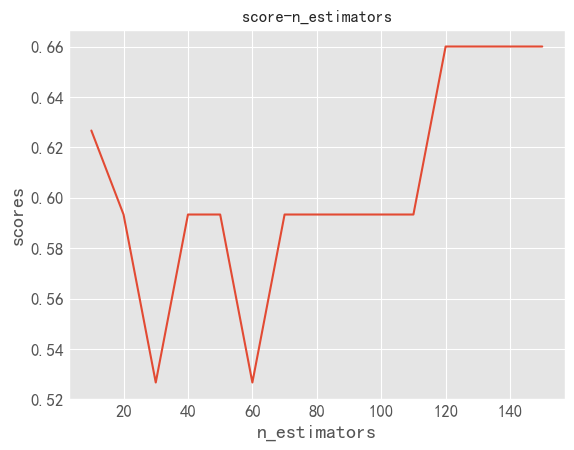
\includegraphics[width=0.95\textwidth]{6.png} 
	\caption{LightGBM原理图} 
	\label{Fig.main6} 
\end{figure}

首先先对表中数据进行特征放缩和特征编码(具体步骤和问题一中数据预处理相同),然后将数据按照80\%的比例划分为训练集和测试集。接着,定义模型参数并构建LightGBM模型。通过基于GridSearchCV的模型调参,通过对LightGBM模型的参数进行网格搜索,以找到最优的参数组合来训练模型,进而提高模型的预测性能。设置一些超参数进行调参,如下表所示:

\begin{table}[H]
    \centering  
    \caption{GridSearchCV对LightGBM调参结果}
    \begin{tabular}{c c c}  
    	\toprule[1.5pt]  
    	参数 & 取值范围 & 最优结果 \\  
    	\midrule[1pt]    
    	max\_depth			&  [4, 7, 10]       & 7   \\
        min\_child\_samples &  [18, 20, 22]     & 22  \\ 
        n\_estimators       &  [10, 70, 130]    & 10  \\
        num\_leaves         &  [300, 600, 900]  & 300 \\
    	\toprule[1.5pt]  
    \end{tabular}  
\end{table} 

基于上表最优参数训练LightGBM模型,再计算模型预测结果与实际值之间的均方误差和平均绝对误差,公式原理为:

\begin{equation}
    MAE=\frac{1}{n}\sum\limits_{i=1}^{n}{\left| {{x}_{i}}-{{\overline{x}}_{i}} \right|}.
\end{equation}

\begin{equation}
    MSE=\frac{1}{n}\sum\limits_{i=1}^{n}{{{({{x}_{i}}-{{\overline{x}}_{i}})}^{2}}}.
\end{equation}
其中,${{x}_{i}}$为第$i$个样本的实际值,${{\overline{x}}_{i}}$为第$i$个样本的预测值,$n$为样本数量,与平均绝对误差相比,均方误差对预测误差较大的样本更加敏感,因为它对误差取平方,使得误差较大的样本对平均误差的影响更大,并分别输出结果如下:

\begin{table}[H]
    \centering  
    \caption{LightGBM评价结果}
    \begin{tabular}{c c c}  
    	\toprule[1.5pt]  
    	标签序号 & MAE & MSE \\  
    	\midrule[1pt]    
        第六主成分特征 & 0.3053	& 0.1391  \\
    	\toprule[1.5pt]  
    \end{tabular}  
\end{table} 

对于MAE和MSE的范围都是$[0,+\infty )$,当预测值和真实值完全吻合时等于0,即完美模型;误差越大,该值越大。即这两个值越小模型精度越高。从上表评价指标可以看到 LightGBM模型的训练效果十分优良,能够充分的得到11个患者特征与15个主成分的情况。



\subsubsection{模型求解}




基于上一问新药组和原有药物组关于第六个主成分特征表现出显著差异,为确定是由于新药造成还是其他因素造成,要对不同生命体征指标对应的特征重要性打分。利用上面训练好的LightGBM模型得到数据可视化图如下:
 
\begin{figure}[H] % 这个H不要动!
	\centering % 不要动!
	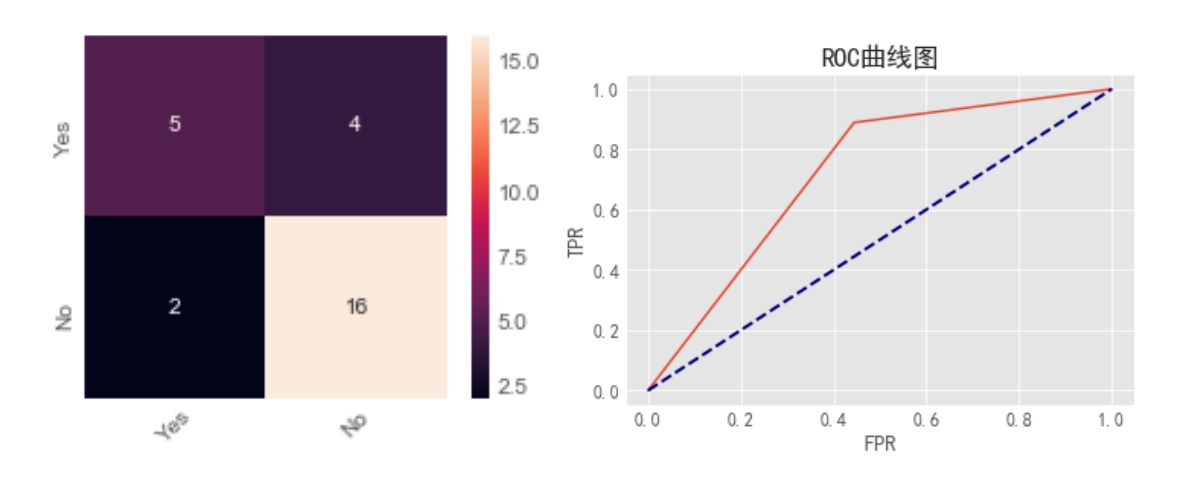
\includegraphics[width=0.95\textwidth]{7.png} 
	\caption{生命体征的显著主成分对应的特征重要性打分} 
	\label{Fig.main7} 
\end{figure} 

分析上图, 横坐标为可能的影响因素(即特征名), 纵坐标为特征重要 性打分, 通过条形图的形式展示了每个特征对应的重要性分值, 从上图发现镇静药的类别在不同因素的影响中重要性程度并不高, 而是与个人的年龄、身高、体重这些客观因素的关联性更大,对于性别、有无既往史、有无手术史、是否酗酒关联性很小,对是否吸烟、有无晕动史、有无ponv之间甚至没有关联。这较为直观的解释了不同药组在生命体征第六主成分上存在显著差异的原因,但从整体上分析新药物对总的生命体征的影响是不大的,甚至比不上客观因素(年龄、身高、体重)的影响,这与实际情况也是吻合的,不同的药物对于生命体征的存在一定的可控的影响。这个结论表明生命体征数据表现出的差异和新药物没有特别强的关联性, 新药物是具有 一定的可信度的,可以正常使用,同时新药和原有药物之间也没有很大的差异性。